
\documentclass[openany, amssymb, psamsfonts]{amsart}
\usepackage{mathrsfs,comment}
\usepackage[usenames,dvipsnames]{color}
\usepackage[normalem]{ulem}
\usepackage{url}
\usepackage{tikz}
\usepackage{tkz-euclide}
\usepackage{lipsum}
\usepackage{marvosym}
\usepackage[all,arc,2cell]{xy}
\UseAllTwocells
\usepackage{enumerate}
\newcommand{\bA}{\mathbf{A}}
\newcommand{\bB}{\mathbf{B}}
\newcommand{\bC}{\mathbf{C}}
\newcommand{\bD}{\mathbf{D}}
\newcommand{\bE}{\mathbf{E}}
\newcommand{\bF}{\mathbf{F}}
\newcommand{\bG}{\mathbf{G}}
\newcommand{\bH}{\mathbf{H}}
\newcommand{\bI}{\mathbf{I}}
\newcommand{\bJ}{\mathbf{J}}
\newcommand{\bK}{\mathbf{K}}
\newcommand{\bL}{\mathbf{L}}
\newcommand{\bM}{\mathbf{M}}
\newcommand{\bN}{\mathbf{N}}
\newcommand{\bO}{\mathbf{O}}
\newcommand{\bP}{\mathbf{P}}
\newcommand{\bQ}{\mathbf{Q}}
\newcommand{\bR}{\mathbf{R}}
\newcommand{\bS}{\mathbf{S}}
\newcommand{\bT}{\mathbf{T}}
\newcommand{\bU}{\mathbf{U}}
\newcommand{\bV}{\mathbf{V}}
\newcommand{\bW}{\mathbf{W}}
\newcommand{\bX}{\mathbf{X}}
\newcommand{\bY}{\mathbf{Y}}
\newcommand{\bZ}{\mathbf{Z}}

%% blackboard bold math capitals
\newcommand{\bbA}{\mathbb{A}}
\newcommand{\bbB}{\mathbb{B}}
\newcommand{\bbC}{\mathbb{C}}
\newcommand{\bbD}{\mathbb{D}}
\newcommand{\bbE}{\mathbb{E}}
\newcommand{\bbF}{\mathbb{F}}
\newcommand{\bbG}{\mathbb{G}}
\newcommand{\bbH}{\mathbb{H}}
\newcommand{\bbI}{\mathbb{I}}
\newcommand{\bbJ}{\mathbb{J}}
\newcommand{\bbK}{\mathbb{K}}
\newcommand{\bbL}{\mathbb{L}}
\newcommand{\bbM}{\mathbb{M}}
\newcommand{\bbN}{\mathbb{N}}
\newcommand{\bbO}{\mathbb{O}}
\newcommand{\bbP}{\mathbb{P}}
\newcommand{\bbQ}{\mathbb{Q}}
\newcommand{\bbR}{\mathbb{R}}
\newcommand{\bbS}{\mathbb{S}}
\newcommand{\bbT}{\mathbb{T}}
\newcommand{\bbU}{\mathbb{U}}
\newcommand{\bbV}{\mathbb{V}}
\newcommand{\bbW}{\mathbb{W}}
\newcommand{\bbX}{\mathbb{X}}
\newcommand{\bbY}{\mathbb{Y}}
\newcommand{\bbZ}{\mathbb{Z}}

%% script math capitals
\newcommand{\sA}{\mathscr{A}}
\newcommand{\sB}{\mathscr{B}}
\newcommand{\sC}{\mathscr{C}}
\newcommand{\sD}{\mathscr{D}}
\newcommand{\sE}{\mathscr{E}}
\newcommand{\sF}{\mathscr{F}}
\newcommand{\sG}{\mathscr{G}}
\newcommand{\sH}{\mathscr{H}}
\newcommand{\sI}{\mathscr{I}}
\newcommand{\sJ}{\mathscr{J}}
\newcommand{\sK}{\mathscr{K}}
\newcommand{\sL}{\mathscr{L}}
\newcommand{\sM}{\mathscr{M}}
\newcommand{\sN}{\mathscr{N}}
\newcommand{\sO}{\mathscr{O}}
\newcommand{\sP}{\mathscr{P}}
\newcommand{\sQ}{\mathscr{Q}}
\newcommand{\sR}{\mathscr{R}}
\newcommand{\sS}{\mathscr{S}}
\newcommand{\sT}{\mathscr{T}}
\newcommand{\sU}{\mathscr{U}}
\newcommand{\sV}{\mathscr{V}}
\newcommand{\sW}{\mathscr{W}}
\newcommand{\sX}{\mathscr{X}}
\newcommand{\sY}{\mathscr{Y}}
\newcommand{\sZ}{\mathscr{Z}}


\renewcommand{\phi}{\varphi}
\renewcommand{\emptyset}{\O}

\newcommand{\abs}[1]{\lvert #1 \rvert}
\newcommand{\norm}[1]{\lVert #1 \rVert}
\newcommand{\sm}{\setminus}


\newcommand{\sarr}{\rightarrow}
\newcommand{\arr}{\longrightarrow}

\newcommand{\hide}[1]{{\color{red} #1}} % for instructor version
%\newcommand{\hide}[1]{} % for student version
\newcommand{\com}[1]{{\color{blue} #1}} % for instructor version
%\newcommand{\com}[1]{} % for student version
\newcommand{\meta}[1]{{\color{green} #1}} % for making notes about the script that are not intended to end up in the script
%\newcommand{\meta}[1]{} % for removing meta comments in the script

\DeclareMathOperator{\ext}{ext}
\DeclareMathOperator{\ho}{hole}
%%% hyperref stuff is taken from AGT style file
\usepackage{hyperref}  
\hypersetup{%
  bookmarksnumbered=true,%
  bookmarks=true,%
  colorlinks=true,%
  linkcolor=blue,%
  citecolor=blue,%
  filecolor=blue,%
  menucolor=blue,%
  pagecolor=blue,%
  urlcolor=blue,%
  pdfnewwindow=true,%
  pdfstartview=FitBH}   
  
\let\fullref\autoref
%
%  \autoref is very crude.  It uses counters to distinguish environments
%  so that if say {lemma} uses the {theorem} counter, then autrorefs
%  which should come out Lemma X.Y in fact come out Theorem X.Y.  To
%  correct this give each its own counter eg:
%                 \newtheorem{theorem}{Theorem}[section]
%                 \newtheorem{lemma}{Lemma}[section]
%  and then equate the counters by commands like:
%                 \makeatletter
%                   \let\c@lemma\c@theorem
%                  \makeatother
%
%  To work correctly the environment name must have a corrresponding 
%  \XXXautorefname defined.  The following command does the job:
%
\def\makeautorefname#1#2{\expandafter\def\csname#1autorefname\endcsname{#2}}
%
%  Some standard autorefnames.  If the environment name for an autoref 
%  you need is not listed below, add a similar line to your TeX file:
%  
%\makeautorefname{equation}{Equation}%
\def\equationautorefname~#1\null{(#1)\null}
\makeautorefname{footnote}{footnote}%
\makeautorefname{item}{item}%
\makeautorefname{figure}{Figure}%
\makeautorefname{table}{Table}%
\makeautorefname{part}{Part}%
\makeautorefname{appendix}{Appendix}%
\makeautorefname{chapter}{Chapter}%
\makeautorefname{section}{Section}%
\makeautorefname{subsection}{Section}%
\makeautorefname{subsubsection}{Section}%
\makeautorefname{theorem}{Theorem}%
\makeautorefname{thm}{Theorem}%
\makeautorefname{excercise}{Exercise}%
\makeautorefname{cor}{Corollary}%
\makeautorefname{lem}{Lemma}%
\makeautorefname{prop}{Proposition}%
\makeautorefname{pro}{Property}
\makeautorefname{conj}{Conjecture}%
\makeautorefname{defn}{Definition}%
\makeautorefname{notn}{Notation}
\makeautorefname{notns}{Notations}
\makeautorefname{rem}{Remark}%
\makeautorefname{quest}{Question}%
\makeautorefname{exmp}{Example}%
\makeautorefname{ax}{Axiom}%
\makeautorefname{claim}{Claim}%
\makeautorefname{ass}{Assumption}%
\makeautorefname{asss}{Assumptions}%
\makeautorefname{con}{Construction}%
\makeautorefname{prob}{Problem}%
\makeautorefname{warn}{Warning}%
\makeautorefname{obs}{Observation}%
\makeautorefname{conv}{Convention}%


%
%                  *** End of hyperref stuff ***

%theoremstyle{plain} --- default
\newtheorem{thm}{Theorem}[section]
\newtheorem{cor}{Corollary}[section]
\newtheorem{exercise}{Exercise}
\newtheorem{prop}{Proposition}[section]
\newtheorem{lem}{Lemma}[section]
\newtheorem{prob}{Problem}[section]
\newtheorem{conj}{Conjecture}[section]
%\newtheorem{ass}{Assumption}[section]
%\newtheorem{asses}{Assumptions}[section]

\theoremstyle{definition}
\newtheorem{defn}{Definition}[section]
\newtheorem{ass}{Assumption}[section]
\newtheorem{asss}{Assumptions}[section]
\newtheorem{ax}{Axiom}[section]
\newtheorem{con}{Construction}[section]
\newtheorem{exmp}{Example}[section]
\newtheorem{notn}{Notation}[section]
\newtheorem{notns}{Notations}[section]
\newtheorem{pro}{Property}[section]
\newtheorem{quest}{Question}[section]
\newtheorem{rem}{Remark}[section]
\newtheorem{warn}{Warning}[section]
\newtheorem{sch}{Scholium}[section]
\newtheorem{obs}{Observation}[section]
\newtheorem{conv}{Convention}[section]

%%%% hack to get fullref working correctly
\makeatletter
\let\c@obs=\c@thm
\let\c@cor=\c@thm
\let\c@prop=\c@thm
\let\c@lem=\c@thm
\let\c@prob=\c@thm
\let\c@con=\c@thm
\let\c@conj=\c@thm
\let\c@defn=\c@thm
\let\c@notn=\c@thm
\let\c@notns=\c@thm
\let\c@exmp=\c@thm
\let\c@ax=\c@thm
\let\c@pro=\c@thm
\let\c@ass=\c@thm
\let\c@warn=\c@thm
\let\c@rem=\c@thm
\let\c@sch=\c@thm
\let\c@equation\c@thm
\numberwithin{equation}{section}
\makeatother

\bibliographystyle{plain}

%--------Meta Data: Fill in your info------
\title{University of Chicago Calculus IBL Course}

\author{Agustin Esteva}

\date{Apr 12. 2024}

\begin{document}

\begin{abstract}

16310's Script 16.\\ Let me know if you see any errors! Contact me at aesteva@uchicago.edu.


\end{abstract}

\maketitle

\tableofcontents

\setcounter{section}{1}
\section*{Definition 1.1: $\pi$}
\begin{defn}
We define $\pi$ is twice the area of a unit semicircle:
\[\pi = 2 \cdot \int_{-1}^1\sqrt{1 - x^2}\]
\end{defn}

\section*{Definition 1.2: Sector Area}
\begin{defn}
Define $A(x): [-1,1]\to \bbR$ as the area seen in Figure 1 as \[A(x) = \frac{x \sqrt{1-x^2}}{2} + \cdot \int_{x}^1\sqrt{1 - t^2}\;dt\]
\begin{figure}[h!]
    \centering
    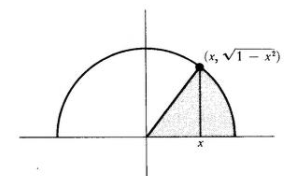
\includegraphics[width=0.5\linewidth]{Images/Trig1.png}
    \caption{Sector Area}
    \label{1.2}
\end{figure}
\end{defn}
\section*{Proposition 1.3}
\begin{prop}
$A(x)$ is differentiable and:
\[A'(x) = \frac{-1}{2\sqrt{1-x^2}}\]
\end{prop}
\vspace{4pt}     \hrule   \vspace{4pt}\begin{proof}:\\
The first term of $A$ is a polynomial and thus integrable, and the second is just a composition of functions, and thus, by the FCT, is differentiable. The rest is left as an exercise by applying the chain rule.
\end{proof}\vspace{4pt}     \hrule   \vspace{4pt}
\section*{Definition 1.4: $\cos(x),\sin(x)$}
\begin{defn}
If $0 < x < \pi$, then $\cos x$ is the unique number in $[ -1, 1]$ such that
\[A (\cos x) =\frac{x}{2};\]
and
\[\sin x =\sqrt{1-\cos^2(x)}\]
\end{defn}

\section*{Theorem 1.5: Derivatives of $\cos$ and $\sin$}
\begin{thm}
If $x\in [0,\pi],$ then:
\[\cos'(x) = -\sin(x)\]
\[\sin'(x) = \cos(x)\]
\end{thm}
\vspace{4pt}     \hrule   \vspace{4pt}\begin{proof}:\\
If $B = 2A,$ then $B(\cos(x)) = x.$ Therefore, $\cos(x)$ is the inverse of $B.$ Note that by Proposition 1.3, $B'(x) = \frac{-1}{\sqrt{1-x^2}}.$ Thus, by Theorem 12.20, 
\begin{align*}
\cos'(x) &= (B^-1)'(x)\\
&= \frac{1}{B'(B^{-1}(x))}\\
&= \frac{1}{B'(\cos(x))}\\
&= \frac{1}{\frac{-1}{\sqrt{1-\cos(x)^2}}}\\
&= -\sqrt{1-\cos(x)^2}\\
&= -\sin(x)
\end{align*}
$\cos'(x) = -\sin(x).$
Moreover, by the chain rule:
\begin{align*}
\sin'(x) &= (\sqrt{1 - \cos^2(x)})'\\
&= -\frac{-2\cos(x)\sin(x)}{2\sqrt{1 - \cos^(x)}}\\
&= \frac{\cos(x)\sin(x)}{\sqrt{1 - \cos^2(x)}}\\
&= \frac{\cos(x)\sin(x)}{\sin(x)}\\
&= \cos(x)
\end{align*}

\section*{Definition 1.6: Trig Functions Galore}
\begin{defn}
Other important trigonometric functions are defined as:
\begin{enumerate}
\item \[\sec(x) = \frac{1}{\cos(x)};\qquad x\neq k\pi + \frac{\pi}{2}\]
\item \[\tan(x) = \frac{\sin(x)}{\cos(x)};\qquad x\neq k\pi + \frac{\pi}{2}\]
\item \[\csc(x) = \frac{1}{\sin(x)};\qquad x\neq k\pi \]
\item \[\cot(x) = \frac{\cos(x)}{\sin(x)};\qquad x\neq k\pi \]
\end{enumerate}
\end{defn}

\section*{Theorem 1.7: Derivatives of Trig Functions Galore}
\begin{thm}
If $1-4$ are defined above, then:
\begin{enumerate}
\item \[\sec'(x) = \sec(x)\tan(x)\]
\item \[\tan'(x) = \sec^2(x)\]
\item \[\csc'(x) = -\csc(x)\cot(x)\]
\[cot'(x) = -\csc^2(x)\]
\end{enumerate}
\end{thm}
\vspace{4pt}     \hrule   \vspace{4pt}\begin{proof}:\\
\begin{enumerate}
\item Because $\sec(x)$ is defined, then $\sec(x) = \frac{1}{\cos(x)}.$ Therefore, by Example 12.9.c:
\begin{align*}
\sec'(x) &= (\frac{1}{\cos(x)})'\\
&= \frac{-\cos'(x)}{\cos^2(x)}\\
&= \frac{\sin(x)}{\cos^2(x)}\\
&= \sec(x)\tan(x)
\end{align*}
\item Because $\sin^2(x) + \cos^2(x) = 1,$ then dividing by $\cos^2(x)$ yields \[\tan^2(x) = \sec^2(x) -1\]
\begin{align*}
2\tan(x)\tan'(x) &= 2\sec(x)\sec'(x)\\
&= 2\sec(x)\sec(x)\tan(x)\\
&= 2\sec^2(x)\tan(x)
\end{align*}
Thus, $\tan'(x) = \sec^2(x)$
\item Parts (3) and (4) are left as an exercise.
\end{enumerate}
\end{proof}\vspace{4pt}     \hrule   \vspace{4pt}

\textit{Note}
We define $\arccos(x), \arcsin(x),$ and $\arctan(x)$ as the inverses of their respective functions, where $\arccos, \arcsin:[-1,1]\to \mathbb{R}$ and $\arctan:\bbR\to [\frac{-\pi}{2}, \frac{\pi}{2}].$

\section*{Theorem 1.8: Derivatives of Inverses}
\begin{thm}
If $x\in [-1,1],$ then:
\begin{enumerate}
\item $\arcsin'(x) = \frac{1}{\sqrt{1-x^2}}$
\item $\arccos'(x) = \frac{-1}{\sqrt{1-x^2}}$
\end{enumerate}
If $x\in \bbR,$ then:\newline
\indent\:\;\textit{(3)} $\arctan'(x) = \frac{1}{1+x^2}$
\end{thm}
\vspace{4pt}     \hrule   \vspace{4pt}\begin{proof}:\\
\begin{enumerate}
\item Using Theorem 12.20:
\begin{align*}
\arcsin'(x) &= \frac{1}{\sin'(\arcsin(x))}\\
&= \frac{1}{\cos(\arcsin(x))}\\
\end{align*}
Note that because $\sin(\arcsin(x))^2 + \cos(\arcsin(x))^2 = 1,$ then $x^2 + \cos(\arcsin(x))^2 = 1.$ Thus, $\cos(\arcsin(x)) = \sqrt{1- x^2}.$ Therefore, $\arcsin'(x) = \frac{1}{\sqrt{1- x^2}}.$
\item The proof is similar to above.
\item Using Theorem 12.20:
\begin{align*}
\arctan'(x) = \frac{1}{\tan'(\arctan(x))}\\
&= \frac{1}{\sec^2(\arctan(x))}
\end{align*}
Note that $\tan^2(x) +1 = \sec^2(x),$ then $\tan^2(\arctan(x)) + 1 = \sec(\arctan(x)).$ Thus, $x^2  + 1 = \sec(\arctan(x)).$
Therefore, $\arctan'(x) = \frac{1}{x^2 +1}.$
\end{enumerate}
\end{proof}\vspace{4pt}     \hrule   \vspace{4pt}


\newpage
\section*{Acknowledgments} 
Spivak!
\begin{thebibliography}{9}




\end{thebibliography}

\end{document}

